\begin{figure}[!p]
    \centering
    \begin{subfigure}[b]{\SideBySidePlotWidth}
        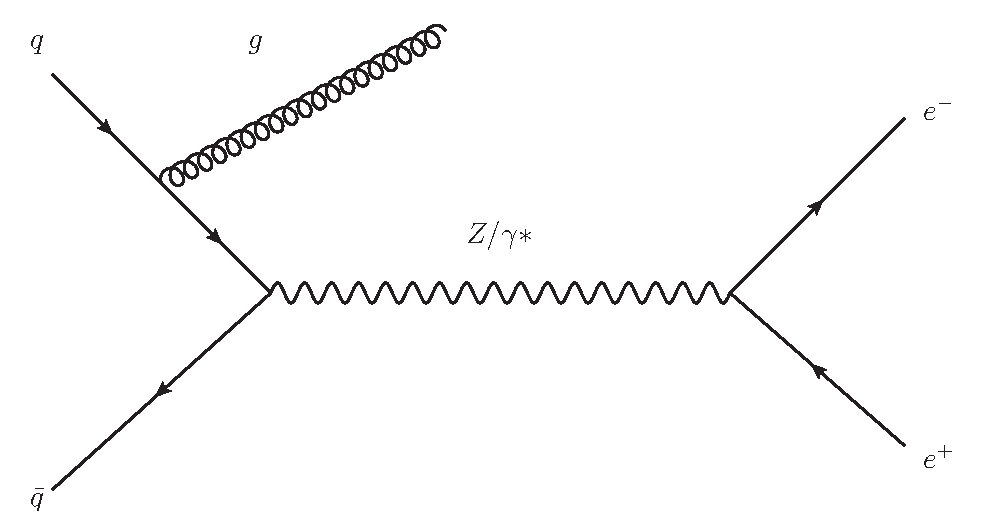
\includegraphics[width=\linewidth]{figures/DYISR.eps}
        \caption{}
        \label{fig:feyn_DYISR}
    \end{subfigure}%
    \begin{subfigure}[b]{\SideBySidePlotWidth}
        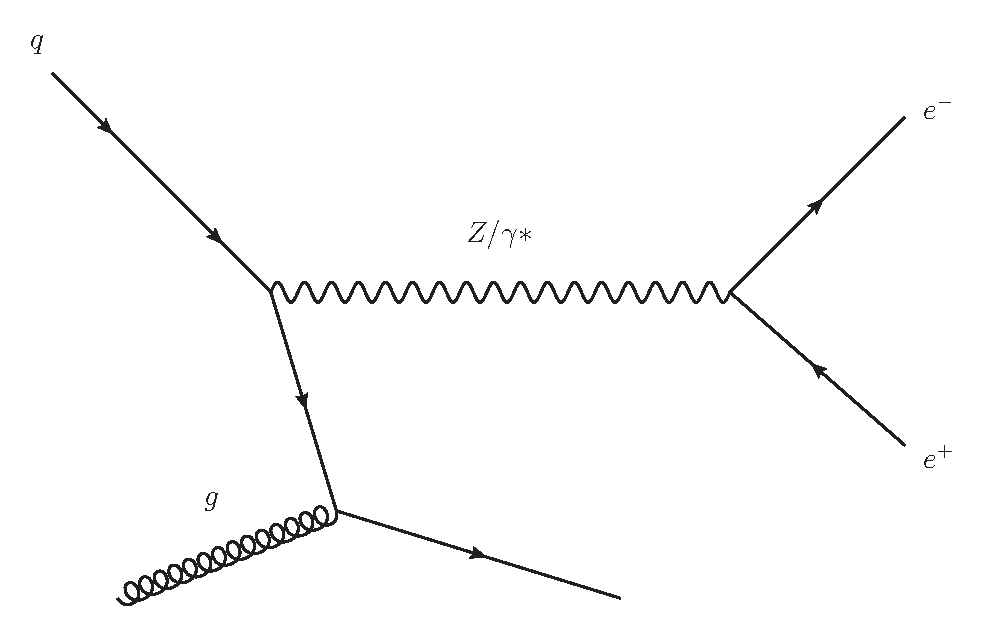
\includegraphics[width=\linewidth]{figures/DYQuarkRadiation.eps}
        \caption{}
        \label{fig:feyn_DYQuarkRadiation}
    \end{subfigure}%
    \hfill
    \begin{subfigure}[b]{\SideBySidePlotWidth}
        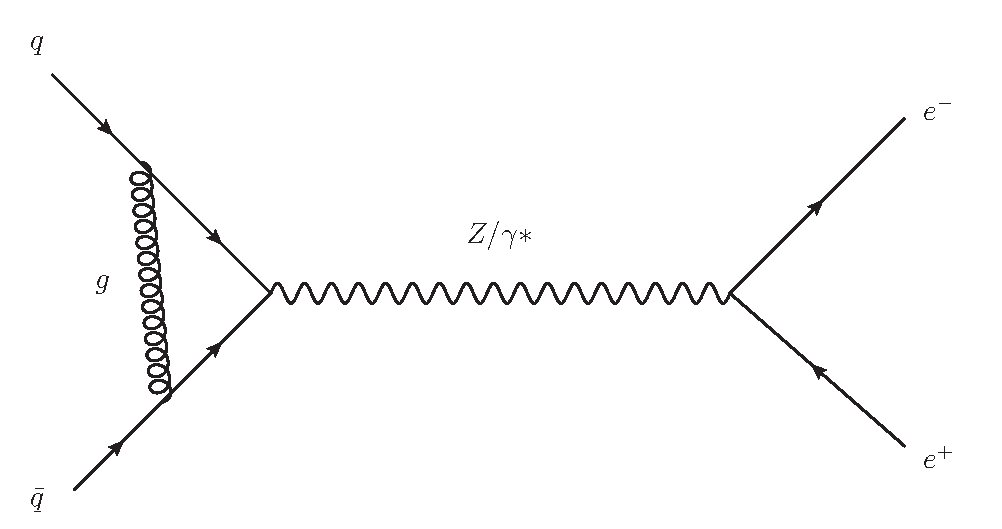
\includegraphics[width=\linewidth]{figures/DYloops.eps}
        \caption{}
        \label{fig:feyn_DYloops}
    \end{subfigure}%
    \begin{subfigure}[b]{\SideBySidePlotWidth}
        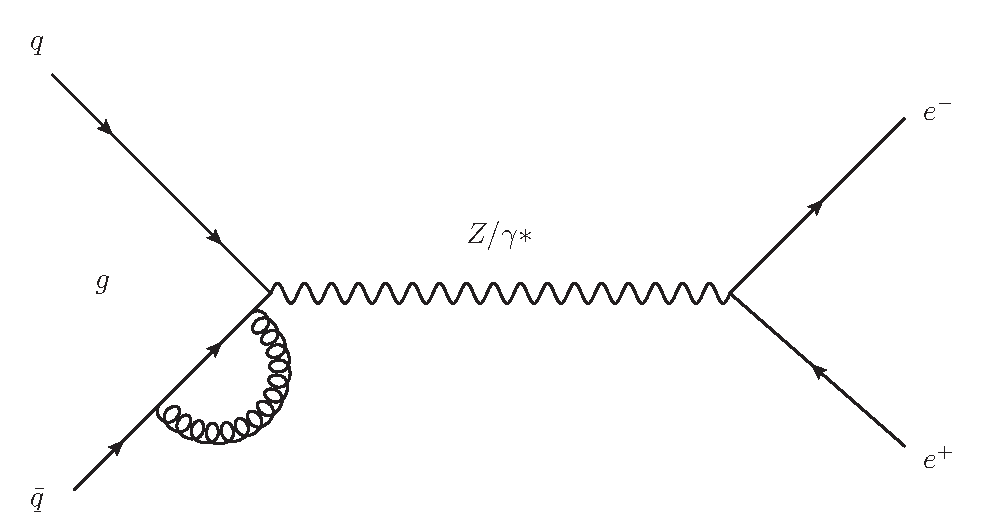
\includegraphics[width=\linewidth]{figures/DYmoreloops.eps}
        \caption{}
        \label{fig:feyn_DYmoreloops}
    \end{subfigure}%

    \caption[
        Higher order DY Feynman diagrams.
    ]{
        Higher order DY Feynman diagrams. \cref{fig:feyn_DYISR} is a example of when a quark incoming radiates a gluon. In \cref{fig:feyn_DYQuarkRadiation} the quark radiates a \Z before interacting with a gluon. In both \cref{fig:feyn_DYloops,fig:feyn_DYmoreloops} the gluons interact with the quarks but are not radiated.
    }
    \label{fig:higher_order_z_diagrams}
\end{figure}